\chapter{Metodología}\label{chapter:methods}

En este capítulo se describe detalladamente el proceso de modelización de los datos y diseño de los algoritmos. Inicialmente, se presenta la descripción CRISP-DM (del inglés, \textit{Cross Industry Standard Process for Data Mining}) con el objetivo de detallar a grandes rasgos el ciclo de vida del proyecto y las diferentes fases. Las siguientes secciones están dedicadas al análisis descriptivo del conjunto de datos a utilizar y la definición de los modelos concebidos para solucionar el problema planteado. 

De manera general, los modelos presentados siguen la metodología \textit{Pointwise}, explicada en el capítulo anterior, transformando el problema de selección de respuestas en un problema de clasificación binaria.

\section{Descripción CRISP-DM}

El proyecto se consta de las siguientes fases:

\begin{itemize}
  \item Comprensión del problema: Definición de necesidades del cliente (comprensión del negocio)
  \item Comprensión de los datos: Estudio y comprensión de los datos
  \item Preparación de los datos: Análisis de los datos y selección de características
  \item Modelado
  \item Evaluación (obtención de resultados)
\end{itemize}

TODO: poner esquema con horas y el ciclo


\section{Descripción del conjunto de datos}

El conjunto de datos Head-QA está organizado en preguntas y respuestas de las categorías: Medicina, Enfermería, Bilogía, Química, Psicología, y Farmacología. Y está dividido en \textit{train}, \textit{development} y \textit{test}. El datset está compuesto por un conjunto de preguntas/respuestas en formato JSON siguiendo la siguientes estructura:

\begin{itemize}
  \item Id: identificador y texto de la pregunta
  \item Ruta: camino a la imagen si lo hay
  \item Respuestas: Una lista con las posibles respuestas
  \item El id de la respuesta correcta
\end{itemize}


\section{Análisis del conjunto de datos}

TODO: Cantidad de muestras por conjunto, palabras más comunes


\subsection{Procesamiento de datos}

Se presentan dos enfoques, el primero aplica arquitecturas propias del aprendizaje supervisado, mientras que el segundo combina técnicas de recuperación de información en arquitecturas de aprendizaje profundo. Cada uno de los enfoques requiere un preprocesamiento y representación de la información diferentes, los cuales se detallan en esta sección.

TODO: Tokenización. Abordar las dos formas de representar los datos


\chapter{Modelos propuestos}\label{chapter:models}

\section{Regresión Logística}

El primer modelo a implementar es un regresor logístico. La simplicidad de este modelo lo hace un buen candidato para establecer un \textit{baseline} entre los modelos de aprendizaje supervisado.


\section{\textit{LSTM} Básico}\label{lstm_t}

La primera propuesta se puede considerar un modelo de aprendizaje profundo relativamente sencillo cuyo objetivo principal es verificar las ventajas que proporcionan las redes recurrentes en la resolución del problema de selección de respuestas. Por esta razón el modelo presentado aprovecha la arquitectura recurrente de la manera más simple posible.

La primera propuesta consiste en una red neuronal recurrente de tipo \textit{LSTM}, la cual recibe como entrada una oración vectorizada. La arquitectura se divide en tres capas: representación de los \textit{tokens}, representación de la oración y predicción de la etiqueta (respuesta correcta). En la Figura \ref{lstm} se presenta la arquitectura de la red correspondiente al modelo matemático que se expone a continuación.

\begin{figure}[!tb]
  \begin{center}    
    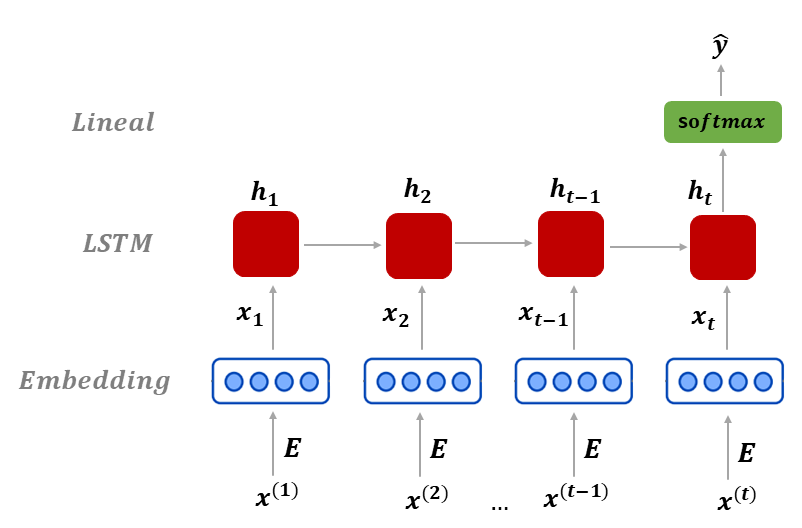
\includegraphics[angle=0, width=0.75\textwidth]{Graphics/lstm2.png} 
  \end{center}
    \caption{Arquitectura del modelo de extracción de relaciones LSTM básico}\label{lstm}
\end{figure}

Sea $S = [x^{(1)}, x^{(2)}, ..., x^{(T)}]$ la representación vectorial de una oración $S$, donde $x^{(t)}$ representa el t-ésimo \textit{token} con $(t = 1, 2, ..., T)$ y $T$, la cantidad de \textit{tokens} de la oración. El modelo puede ser definido formalmente como:

\begin{align}
  x_{t} &= Ex^{(t)} \label{lstm:emb} \\
  \nonumber \\
  i_{t} &= \sigma{(W^{(i)} x_{t} + U^{(i)}h_{t-1})} \label{lstm:ig} \\
  f_{t} &= \sigma{(W^{(f)} x_{t} + U^{(f)}h_{t-1})} \label{lstm:fg} \\
  o_{t} &= \sigma{(W^{(o)} x_{t} + U^{(o)}h_{t-1})} \label{lstm:og} \\
  \tilde{c_{t}} &= \tanh(W^{(c)} x_{t} + U^{(c)}h_{t-1}) \label{lstm:new_memory_generation} \\
  c_{t} &= f_{t}c_{t-1} + i_{t}\tilde{c_{t}} \label{lstm:cell_state} \\
  h_{t} &= o_{t}\tanh{c_{t}} \label{lstm:hidden_state} \\
  \nonumber \\
  \hat{y} &= softmax(Uh_{T} + b) \label{lstm:pred}
\end{align}

En una primera etapa (Ecuación \ref{lstm:emb}), el modelo obtiene una representación más rica semánticamente de cada uno de los \textit{tokens} que conforman una oración. Esto se logra a través de una capa de \textit{embeddings} $E$ que transforma cada \textit{token} $x^{(t)}$ en un vector $x_{t}$ $\in$ ${\mathbb{R}} ^{d}$, donde $d$ es la dimensión de los \textit{embeddings} que constituye un hiperparámetro del modelo.

En la segunda etapa (Ecuaciones \ref{lstm:ig} - \ref{lstm:hidden_state}), el modelo procesa la secuencia de \textit{tokens} para obtener una representación final de la oración. Esto se logra con la inclusión de una capa \textit{LSTM}, la cual analiza de manera secuencial cada una de las salidas $x_{t}$ de la capa de \textit{embeddings}. El centro de una red \textit{LSTM} es el funcionamiento de sus celdas, una red \textit{LSTM} tiene tantas celdas como \textit{tokens} tiene una oración. Las Ecuaciones \ref{lstm:ig} - \ref{lstm:hidden_state} describen el comportamiento de una celda de la red \textit{LSTM}. En la tabla \ref{tab:cell_state} se describe la notación empleada.

\begin{table}[!tb]
  \center \caption{Descripción de símbolos utilizados en una red \textit{LSTM}}
    \begin{center}
      \begin{tabular}{|c|l|}
        \hline
        \textbf{Símbolo} & \textbf{Significado}\\
        \hline
        $x_{t}$ & entrada a la celda \textit{LSTM} en el paso $t$ \\
        $h_{t-1}$ & salida de la celda \textit{LSTM} en el paso $t-1$ \\
        $i_{t}$ & valor de la \textit{input gate} en el paso $t$\\
        $f_{t}$	& valor de la \textit{forget gate} en el paso $t$ \\
        $o_{t}$	& valor de la \textit{output gate} en el paso $t$\\
        $\sigma$ & función sigmoidal\\
        $W^{(\alpha)}$ & pesos de $x_{t}$ en $\alpha_t$ ($\alpha = {i, f, o}$) \\
        $U^{(\alpha)}$ & pesos de $h_{t-1}$ en $\alpha_t$ ($\alpha = {i, f, o}$) \\
        $\tilde{c_{t}}$ & candidato a \textit{cell state} en el paso $t$\\
        $c_{t}$ & \textit{cell state} en el paso $t$ \\
        $h_{t}$ & salida final de la celda \textit{LSTM} en el paso $t$ \\
        $h_{T}$ & salida final de la celda \textit{LSTM} en el último paso $T$ \\
        \hline
        \end{tabular}
    \end{center}
    \label{tab:cell_state}
\end{table}

Una celda \textit{LSTM} está compuesta por tres componentes fundamentales:
\begin{itemize}
  \item La \textit{input gate}, en español "válvula de entrada", expresada en la Ecuación \ref{lstm:ig}, tiene la función de determinar qué información debe estar presente en el estado de la celda (en inglés, \textit{cell state}) representado por $c_{t}$, teniendo en cuenta la salida final de la celda anterior $h_{t-1}$.
  \item La \textit{forget gate}, en español "válvula del olvido", representada en la Ecuación \ref{lstm:fg}, tiene la función de determinar qué información es irrelevante en el estado de la celda $c_{t}$; funciona de manera análoga a la \textit{input gate}.
  \item La \textit{output gate}, en español "válvula de salida", representada en la Ecuación \ref{lstm:og}, tiene la función de determinar el nivel de activación del estado $c_{t}$ para la salida final.
\end{itemize}

En todos estos casos, se utiliza como función de activación la función sigmoide $\sigma$ con el propósito de que los valores sean positivos y se encuentren entre 0 y 1; de esa manera es sencillo interpretar la importancia de las componentes.

La Ecuación \ref{lstm:new_memory_generation}, conocida como \textit{new memory generation} o \textit{candidate cell}, calcula un estado recurrente temporal $\tilde{c_{t}}$ teniendo en cuenta la entrada $x_{t}$ y el estado anterior $h_{t-1}$. En este caso, para superar el problema de \textit{vanishing gradient}\footnote{https://towardsdatascience.com/the-vanishing-gradient-problem-69bf08b15484} se necesita una función de activación cuya segunda derivada pueda mantenerse durante un largo rango antes de llegar a cero, razón por la cual se utiliza la tangente.

En la Ecuación \ref{lstm:cell_state} se calcula el estado de la celda actual $c_{t}$ teniendo en cuenta qué debe olvidar del estado previo a través de la expresión $f_{t}*c_{t-1}$ y qué debe considerar del estado actual temporal representado en la expresión $i_{t}*\tilde{c_{t}}$. En la Ecuación \ref{lstm:hidden_state} se toma el estado de la celda $c_{t}$ y la \textit{output gate} $o_{t}$ para determinar qué información queda contenida en el estado último de la celda $h_{t}$.

Es importante destacar que los parámetros $E$, $W^{(i)}$, $W^{(f)}$, $W^{(o)}$, $W^{(c)}$, $U^{(i)}$, $U^{(f)}$, $U^{(o)}$, $U^{(c)}$ y $U$ son aprendidos durante la etapa de entrenamiento en el proceso de \textit{backpropagation}.

Las operaciones presentadas en las ecuaciones \ref{lstm:ig} - \ref{lstm:hidden_state} son ejecutadas $T$ veces, por cada uno de los \textit{tokens} que conforman una oración. Tras el análisis del último \textit{token} $T$, el estado final $h_{T}$ constituye una representación de la oración $S$. Finalmente, una capa lineal (Ecuación \ref{lstm:pred}) utiliza la representación de la oración obtenida $h_{T}$ para predecir la relación $\hat{y}$ existente en la oración. Esta salida se convierte en una distribución de probabilidades empleando la función \textit{softmax}. Esta operación, a diferencia de las ecuaciones anteriores, solo se aplica una vez al estado final $h_{T}$ de la capa \textit{LSTM}.

La sencillez arquitectónica del modelo permite que se pueda utilizar como base para la comparación con otros modelos más complejos que serán abordados a continuación.

\section{\textit{BiLSTM+Att}}\label{bilstm_t}

El tercer modelo propuesto tiene una arquitectura más compleja que el anterior consistiendo, esencialmente, en una red \textit{BiLSTM} integrada con un mecanismo de atención.

En este caso, se adiciona el uso de un modelo del lenguaje (en inglés, \textit{language model})  (\cite{mikolov-2016-fastext}) pre-entrenado en un conjunto de documentos en idioma español con el propósito de ganar riqueza semántica en la representación de la oración. Utilizar un modelo pre-entrenado ofrece la posibilidad de aprovechar el conocimiento del lenguaje contenido en la representación de las palabras (a través de los \textit{embeddings} pre-entrenados en una tarea auxiliar) en nuestra tarea específica que, en este caso, es la selección de respuestas. El modelo del lenguaje empleado es el presentado por \cite{mikolov-2016-fastext}, entrenado sobre un conjunto de artículos médicos tomados de la biblioteca electrónica \textit{Scielo}\footnote{https://scielo.isciii.es/scielo.php} tomados de \cite{2019-medical-fastext}.

Las redes recurrentes unidireccionales en general, en el análisis de una palabra, tienen en cuenta solo las palabras anteriores (o posteriores), sin embargo sería útil que al hallar la representación de una palabra se tuviera en cuenta tanto las palabras que aparecen antes como las que aparecen después en una oración. Por esta razón se decide utilizar una capa \textit{BiLSTM}, esto posibilita que en cada estado de una secuencia, la red tenga una visión completa y consecutiva de todos los estados anteriores y posteriores. Se propone la inclusión de una capa de atención pues podría ayudar al modelo a darle más peso a ciertas palabras en la oración que pueden ser determinantes en la predicción.

En la figura \ref{bilstm} se expone la arquitectura de la red correspondiente al modelo matemático que se presenta en esta sección. Seguidamente se presenta una parte de la representación formal del modelo.

\begin{figure}[!tb]
  \begin{center}
    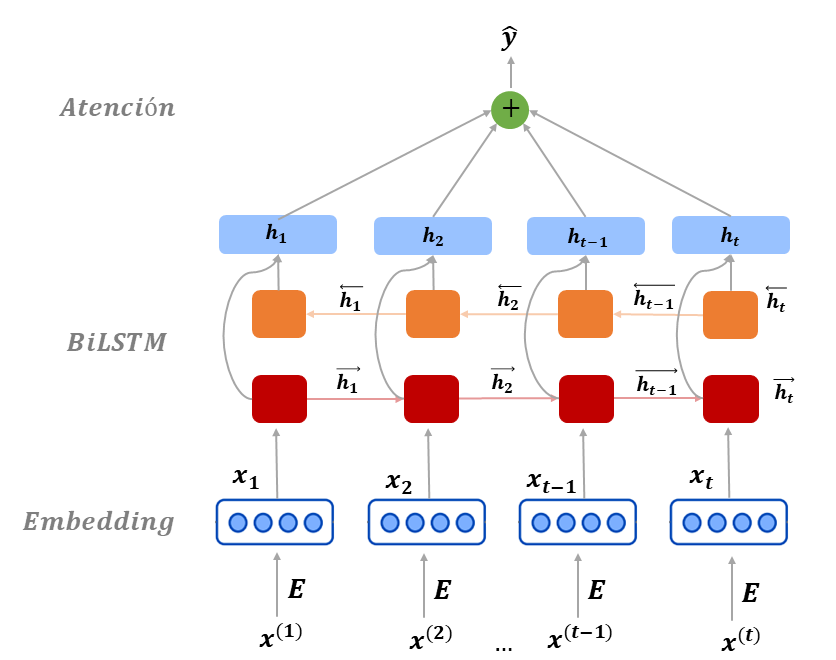
\includegraphics[angle=0, width=0.75\textwidth]{Graphics/bilstm.png}
  \end{center}
    \caption{Arquitectura del modelo de extracción de relaciones \textit{BiLSTM+Att}}\label{bilstm}
\end{figure}

Sea $S = [x^{(1)}, x^{(2)}, ..., x^{(T)}]$, donde $x^{(t)}$ representa el t-ésimo \textit{token} con $(t = 1, 2, ..., T)$ y $T$, la cantidad de \textit{tokens} de la oración $S$. El modelo puede ser definido formalmente como:

\begin{align}
  x_{t} &= Ex^{(t)} \label{bilstm:emb}\\
  \nonumber \\
  \overrightarrow{i_{t}} &= \sigma{(\overrightarrow{W^{(i)}} x_{t} + \overrightarrow{U^{(i)}}\overrightarrow{h_{t-1}})} \label{bilstm:ig} \\
  \overrightarrow{f_{t}} &= \sigma{(\overrightarrow{W^{(f)}} x_{t} + \overrightarrow{U^{(f)}}\overrightarrow{h_{t-1}})} \label{bilstm:fg} \\
  \overrightarrow{o_{t}} &= \sigma{(\overrightarrow{W^{(o)}} x_{t} + \overrightarrow{U^{(o)}}\overrightarrow{h_{t-1}})} \label{bilstm:og} \\
  \overrightarrow{\tilde{c_{t}}} &= \tanh(\overrightarrow{W^{(c)}} x_{t} + \overrightarrow{U^{(c)}}\overrightarrow{h_{t-1}}) \label{bilstm:new_memory_cell}
\end{align}

\begin{align}
  \overrightarrow{c_{t}} &= \overrightarrow{f_{t}}\overrightarrow{c_{t-1}} + \overrightarrow{i_{t}}\overrightarrow{\tilde{c_{t}}} \label{bilstm:cell_state} \\
  \overrightarrow{h_{t}} &= \overrightarrow{o_{t}}\tanh{\overrightarrow{c_{t}}} \label{bilstm:hidden_state}\\
  \nonumber \\
  \overleftarrow{i_{t}} &= \sigma{(\overleftarrow{W^{(i)}} x_{t} + \overleftarrow{U^{(i)}}\overleftarrow{h_{t+1}})} \label{bilstml:ig} \\
  \overleftarrow{f_{t}} &= \sigma{(\overleftarrow{W^{(f)}} x_{t} + \overleftarrow{U^{(f)}}\overleftarrow{h_{t+1}})} \label{bilstml:fg} \\
  \overleftarrow{o_{t}} &= \sigma{(\overleftarrow{W^{(o)}} x_{t} + \overleftarrow{U^{(o)}}\overleftarrow{h_{t+1}})} \label{bilstml:og} \\
  \overleftarrow{\tilde{c_{t}}} &= \tanh(\overleftarrow{W^{(c)}} x_{t} + \overleftarrow{U^{(c)}}\overleftarrow{h_{t+1}}) \label{bilstml:new_memory_cell} \\
  \overleftarrow{c_{t}} &= \overleftarrow{f_{t}}\overleftarrow{c_{t+1}} + \overleftarrow{i_{t}}\overleftarrow{\tilde{c_{t}}} \label{bilstml:cell_state} \\
  \overleftarrow{h_{t}} &= \overleftarrow{o_{t}}\tanh{\overleftarrow{c_{t}}} \label{bilstml:hidden_state}
\end{align}

El modelo contiene una primera capa de \textit{embeddings} pre-entrenada que transforma el \textit{word index} en una representación más rica semánticamente representada como un vector $x_{t} \in {\mathbb{R}} ^{d}$, donde $d$ es la dimensión de los \textit{embeddings} que constituye un hiperparámetro del modelo. Es importante aclarar que la Ecuación \ref{bilstm:emb} luce exactamente como la Ecuación \ref{lstm:emb} correspondiente al modelo anterior, la diferencia se encuentra en que en el modelo \textit{LSTM} los pesos de la capa de \textit{embeddings} $E$ se aprenden durante la etapa de entrenamiento, mientras que, en este caso, los pesos que se utilizan pertenecen a \textit {embeddings} pre-entrenados tomados de \cite{2019-medical-fastext} que ya contienen un conocimiento del idioma español y del dominio médico específicamente, adquirido previamente.

Una segunda capa está conformada por una red \textit{Bi-LSTM}, la cual permite tener en cuenta para el cómputo de un estado no solo las palabras anteriores sino también las siguientes. Las Ecuaciones \ref{bilstm:ig} - \ref{bilstm:hidden_state} representan la \textit{LSTM} orientada de izquierda a derecha, que comienza en el principio de la oración y concluye en el final, mientras que en las Ecuaciones \ref{bilstml:ig} - \ref{bilstml:hidden_state} representan la \textit{LSTM} orientada en sentido contrario, de derecha a izquierda. La arquitectura de la red bidireccional es muy similar a la presentada en el modelo anterior, con la diferencia que se han incluido las flechas para indicar el sentido de la red.

Las ecuaciones serán aplicadas secuencialmente a cada uno de los \textit{tokens} $x^{(t)}$ que conforman una oración $S$. En este caso, a diferencia del modelo presentado anteriormente, en lugar de utilizar solo el último estado $h_{T}$ de la red, se utilizan todos los estados intermedios $h_{t}$  $(t = 1, 2, ..., T)$. De manera que, por cada capa \textit{LSTM}, se obtiene un conjunto de estados $h_{1}, h_{2}, ..., h_{T}$.

En el caso de la red \textit{BiLSTM} se obtienen dos conjuntos de estados. Se utiliza la notación $\overrightarrow{h_{t}}$ y $\overleftarrow{h_{t}}$ como referencia al t-ésimo estado de la red izquiera-derecha y derecha-izquierda respectivamente. Por lo que, los dos conjuntos de estados intermedios se representan como $\overrightarrow{h_{1}}, \overrightarrow{h_{2}}, ... \overrightarrow{h_{T}}$ y $\overleftarrow{h_{1}}, \overleftarrow{h_{2}}, ... \overleftarrow{h_{T}}$. En el resto del modelo, en función de ganar claridad en la escritura, se utilizará $\overrightarrow{h_{t}}$ y  $\overleftarrow{h_{t}}$ para denotar los estados intermedios de forma genérica.

\begin{align}
  h_{t} &= [\overrightarrow{h_{t}} \oplus \overleftarrow{h_{t}}] \label{bilstm:concat} \\
  W &= \tanh{(IW_{a} + B)} \label{bilstm:dense} \\
  A &= sofmax(W) \label{bilstm:sig} \\
  c &= IA^{T} \label{bilstm:dot} \\
  \hat{y} &= softmax(Uc + b) \label{bilstm:pred}
\end{align}

donde $h_{t} \in {\mathbb{R}} ^{2d}$ es el resultado de concatenar $\overrightarrow{h_{t}} \in {\mathbb{R}} ^{d}$ con $\overleftarrow{h_{t}} \in {\mathbb{R}} ^{d}$ y constituye el estado definitivo de la celda $t$, expresado en la Ecuación \ref{bilstm:concat}. La salida de la capa \textit{BiLSTM} constituye entonces, un conjunto de estados $I  = {[h_{1}, h_{2}, ..., h_{T}]}$ con $I \in {\mathbb{R}}^{(T \times 1)}$.

El objetivo de incluir un mecanismo de atención es que el modelo dé mayor peso a aquellas palabras que tienen una mayor influencia en la predicción final. Intuitivamente, lo que se quiere es un vector de pesos con el mismo tamaño $T$ que la cantidad de palabras de la oración. Dicho vector debe poseer en cada componente un número positivo entre 0 y 1 que indique cuán relevante es esa palabra para la clasificación. Por esta razón, la Ecuación \ref{bilstm:dense} toma la salida de la red \textit{BiLSTM}, $I \in {\mathbb{R}}^{(T \times 1)}$, como entrada a una capa densa, donde $W_{a}$ es la matriz aprendida durante la etapa de entrenamiento, con función de activación tangente que obtiene como salida el vector de pesos no normalizado $W$. Con el objetivo de expresar los valores de $W$ en una escala entre 0 y 1 se aplica la función \textit{softmax}, como se muestra en la Ecuación \ref{bilstm:sig}, obteniendo un vector $A$ distribuido probabilísticamente cuyas componentes representan los pesos de atención. En la Ecuación \ref{bilstm:dot} se combina el vector de pesos de atención $A$ con la salida de la capa \textit{BiLSTM} dando como resultado un vector $c$, conocido como vector contexto, que constituye la representación final de la oración. Finalmente, una capa lineal utiliza la representación de la oración obtenida $c$ para predecir la relación $\hat{y}$ existente en la oración. Esta salida se convierte en una distribución de probabilidades empleando la función \textit{softmax}.

\section{\textit{Transfer Learning} basado en BERT}\label{bert_t}

\cite{2018-devlin-bert} plantea que el uso de BERT en el enfoque \textit{fine tuning} obtiene nuevos resultados en el estado del arte en varias tareas de procesamiento del lenguaje natural, entre ellas, el reconocimiento de entidades nombradas y los sistemas pregunta/respuesta.

La diferencia con otros modelos de representación del lenguaje, en cuanto a arquitectura, es que BERT está basado en un \textit{Transformer} bidireccional. En el artículo de \cite{2018-devlin-bert} no se detalla la arquitectura del modelo \textit{Transformer}. Otra diferencia es que modifica la tarea tradicional de \textit{language modeling} sobre la que se entrena introduciendo nuevas tareas. La primera tarea introducida recibe el nombre de \textit{masked language model} y consiste en ocultar palabras aleatorias en un texto y predecir, teniendo en cuenta el contexto, el \textit{token} que corresponde a la posición oculta, mientras que la segunda tarea consiste en, dada una oración en un texto, predecir la oración siguiente.

Los autores de BERT señalan como principal contribución la demostración de la efectividad del pre-entrenamiento bidireccional en la representación del lenguaje sobre las arquitecturas unidireccionales utilizadas hasta ese momento y, además, plantean que con el uso de esta nueva representación se puede reducir la complejidad de la arquitectura del modelo y aún así, obtener mejores resultados.

En esta tesis se propone un modelo que hace uso del modelo de lenguaje aprendido utilizando BERT e incorpora un modelo de predicción simple. La propuesta tiene como objetivo comprobar si los aportes de BERT se pueden extender al idioma español y, específicamente, a la tarea de extracción de relaciones semánticas entre entidades.

\section{QA LSTM}

\section{QA LSTM + CNN}

\section{QA BERT}

\subsection{Especificidad del preprocesamiento}

Con el objetivo de transformar una oración en un vector computacionalmente interpretable, se propuso un preprocesamiento que fue aplicado a los modelos de aprendizaje presentados. Sin embargo, en el caso de BERT, las oraciones no pueden ser traducidas a vectores numéricos de la misma forma que se hizo en las propuestas anteriores, sino que BERT requiere un formato diferente. Con el fin de obtener los resultados esperados, el corpus original siempre debe ser modificado en función de las pautas planteadas por los autores en \cite{2018-devlin-bert}.

BERT define los siguientes \textit{tokens} especiales para la representación de una oración. Dichos \textit{tokens} reciben una interpretación diferente en la etapa de entrenamiento.
\begin{itemize}
  \item \textbf{[CLS]}: Indica el inicio de una oración
  \item \textbf{[SEP]}: Indica el fin de una oración
  \item \textbf{[MASK]}: Se utiliza para denotar \textit{tokens} que deben ser ignorados por el modelo
\end{itemize}

BERT no acepta secuencias de tamaño variable por lo que se recurre a la estrategia de \textit{padding}, en la que se establece un tamaño máximo. Las oraciones que tienen una cantidad menor de \textit{tokens} son completadas con el \textit{token} especial \textbf{[MASK]}, para indicar que esas posiciones deben ser ignoradas.

\section{Implementación}




